\documentclass{sig-alternate}

%Deadline: April 8, 2015
%Call for papers: http://www.computer.org/web/computingnow/swcfp6

\usepackage{url}
\usepackage[table,xcdraw]{xcolor}
\usepackage{eurosym}
\usepackage{amsfonts}
\usepackage{balance}
\usepackage{cite} %this package is awesome - it reorders lists of citations to be in numeric order
\usepackage{pifont}
\usepackage{eqparbox}

% Tables
\usepackage{booktabs}
\usepackage{pbox}
\renewcommand{\arraystretch}{1.2} 
\usepackage{arydshln}
%\renewcommand*\cmidrule{} % No middle lines
%\renewcommand{\arraystretch}{1.5} % Additional spacing with no middle lines
%\renewcommand*\cmidrule{\hdashline[1pt/2pt]}% Dashed middle lines
\renewcommand*\cmidrule{\midrule[0.001em]} % Thin middle lines
%\renewcommand*\cmidrule{\midrule} % Thick middle lines

%Images
%\usepackage[pdftex]{graphicx}
\DeclareGraphicsExtensions{.pdf,.jpg,.png}

\hyphenation{second-ly ap-pen-dix}

\clubpenalty = 10000
\widowpenalty = 10000
\displaywidowpenalty = 10000

\newcommand{\todo}[1]{\textbf{TODO: #1}}
\newcommand{\ms}{LEGO MINDSTORMS EV3}
\newcommand{\mbs}{\textsc{my blocks}}
\newcommand{\mb}{\textsc{my block}}

\newcommand{\ignore}[1]{}

\begin{document}
%\bstctlcite{IEEEexample:BSTcontrol}
%
% paper title
% can use linebreaks \\ within to get better formatting as desired
\title{A Catalog of OO-inspired End-User Smells, \\and Application to \ms~and Kodu}
%\title{Perspectives on End-User Refactoring: Past, Present, and Future}

\numberofauthors{3}
\author{
% 1st. author
\alignauthor
David Hoepelman\\
       \affaddr{Delft University of Technology}\\
       \affaddr{Mekelweg 4}\\
       \affaddr{Delft, the Netherlands}\\
       \email{D.J.Hoepelman@tudelft.nl}
\alignauthor
Kathryn T. Stolee\\
       \affaddr{Department of Computer Science}\\
       \affaddr{Iowa State University}\\
       \affaddr{Ames, IA, U.S.A.}\\
       \email{kstolee@iastate.edu}
\alignauthor
Felienne Hermans\\
       \affaddr{Delft University of Technology}\\
       \affaddr{Mekelweg 4}\\
       \affaddr{Delft, the Netherlands}\\
       \email{f.f.j.hermans@tudelft.nl}
}
%\author{David Hoepelman, Katryn Stolee, Felienne Hermans}

\maketitle


\begin{abstract}
In the workforce today, millions of people program without degrees or professional training in software development. 
These end-user programmers perform a variety of tasks, from combining web information to building models to support business decisions. Software engineering research into code smells has traditionally focused on professionally used object-oriented programming languages, yet these end-user domains and languages also suffer from code smells. 

In this work, we explore recent research in two distinct end-user domains and languages: spreadsheets in Microsoft Excel and web mashups in Yahoo!\ Pipes. Based on existing OO-smells and their applications to these two end-user domains, we distill a catalog of generic end-user smells. 

We demonstrate the broad applicability of the catalog by applying it to two end-user languages not previously targeted by smell detection and refactoring research, both aimed at education: \ms~and Microsoft's Kodu. The results of this application show that indeed OO inspired smells occur in both end-user languages, most commonly we find that small abstractions, duplication and dead code are common. We conclude the paper by proposing new end-users smell, moving beyond the OO paradigm. 
\end{abstract}


\section{Introduction}
End-user programmers are said to outnumber  professional programmers three times over \cite{Scaf2005}.
These end-user programmers perform a wide variety of tasks within their organizations, ranging from creating new web streams to building and maintaining applications in a spreadsheet.
While performing these tasks, end-user programmers face many of the challenges of professional developers, such as identifying faults, debugging, or understanding code written by someone else~\cite{Ko2011}.

Similar to code written by professional developers, end-user artifacts may have a long life-span, the average lifespan of a corporate spreadsheet being five years~\cite{Hermans2011}.
During this long lifespan, end-user artifacts are modified, often by different people.
These properties make them, like source code artifacts, vulnerable to \emph{smells}. 

Smells in end-user programming have been a topic of research over the past few years. Most notable are structural smells in Yahoo!\ Pipes web mashups~\cite{Stolee2011} and  Excel spreadsheets \cite{Hermans2012inter} Experiments in both areas have shown that end-user programmers understand smells, and often prefer versions of their code that are non-smelly \cite{Hermans2012intra, StoleeTSE2013, chambers2013smell}. Alleviating those smells can be achieved with refactoring.

%Refactoring was first introduced as a systematic way to restructure source code and facilitate software evolution and maintenance. Martin Fowler later introduced the concept of code smells \cite{Fowl1999}. Refactoring code is often motivated by noticing a code smell, which signals the opportunity for improvement.

The taxonomy of smells outlined in Fowler's text pertained  to object-oriented (OO) code, and professional programming languages were the focus for at least the first decade of refactoring and code smell research~\cite{Mens:2004:SSR:972215.972286}.

%Like smell definitions refactorings have too been adapted and extended to other  end-user programming paradigms, including web mashups~\cite{Stolee2011, StoleeTSE2013}, Excel spreadsheets~\cite{Hermans2011, Hermans2012inter, hermans2014bumblebee}, and LabVIEW programs~\cite{chambers2013smell}.

Considering the large number of end-user programmers, the longevity of their artifacts and the preference for non-smelly code, supporting end-user programmers in code smell detection is valuable. The applicability of smells, originally created to detect weaknesses in source code, to other domains shows how powerful the concept is. Furthermore, studying the smells in a fresh context provides new insight on how to use smells in software engineering and even suggests new types of smells. 
The contributions of this work are:

\begin{itemize}
	\item Synthesis and catalog of object-oriented-inspired code smells in end-user programs
	\item Application of the catalog to two new end-user domains focused on education: \ms~and Kodu
	\item Identification of future opportunities for smell detection in end-user programming domains, both OO based and more domain specific
\end{itemize}


\section{Background}
\label{sec:background}
In this section we briefly explore the two end-user languages targeted by prior smell research, before presenting the relevant end-user code smells in Section~\ref{sec:smells}.



\begin{figure}
\caption{Microsoft Excel 2013 showing a spreadsheet. Column B and C shows the typical mix of data and calculation. The formula of the selected cell B17 is visible right above the spreadsheet.}
\centering
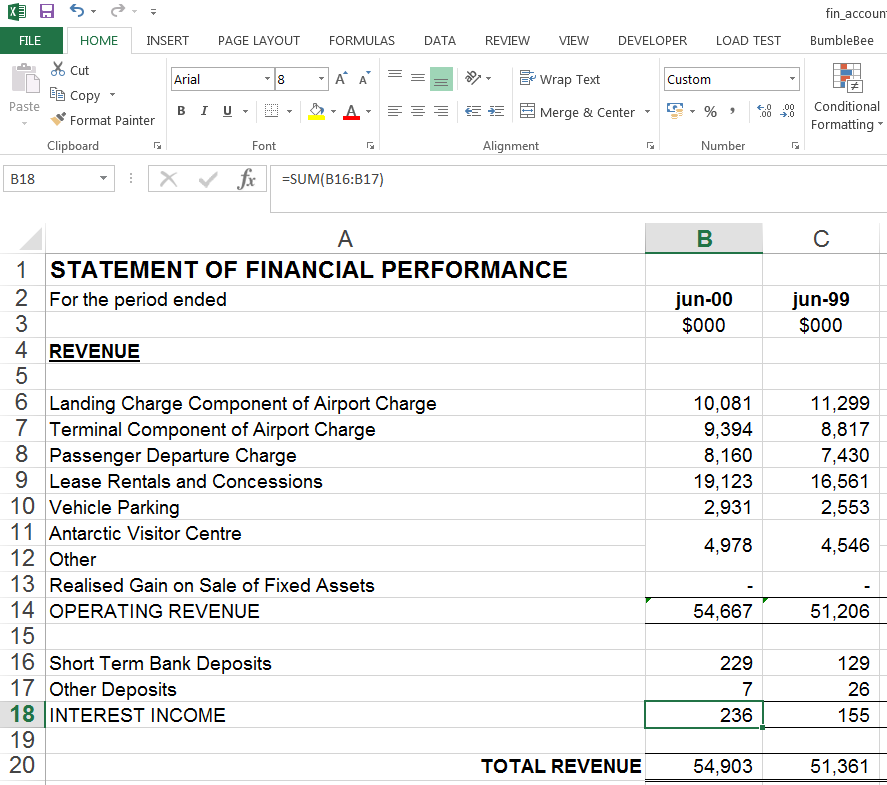
\includegraphics[width=\columnwidth]{img/excel-2}
\label{fig:spreadsheetexample}
%file: fin_accounts from Euses / financial
\end{figure}

\noindent \textbf{Excel:} Spreadsheets are very commonly used in businesses, from inventory administration to educational applications and from scientific modeling to financial systems.
Winston ~\cite{Wins2001} estimates that 90\% of all analysts in industry perform calculations in spreadsheets. 
Microsoft Excel is by far the most used, and therefore most studied, spreadsheet program, but other implementations exists and are similar.

In modern spreadsheet programs, a \textit{cell} can contain a single \textit{formula} which performs a calculation, and a table of cells is bundled in a \textit{worksheet}; an example is shown in Figure~\ref{fig:spreadsheetexample}. 
A \textit{workbook} consist of a collection of worksheets.
Formulas can reference other cells in the same or in different workbooks and worksheets.


\noindent \textbf{Yahoo!\ Pipes:}
Yahoo!\ Pipes is a popular web mashup language and environment with which RSS feed information can be collected and combined from various sources.  Figure~\ref{fig:ypexample} shows an example program. The boxes represent modules connected by wires. 
Abstraction is possible with \emph{subpipe} modules, which allow a programmer to insert a different pipe as a subroutine, appearing like a standard module. 

\begin{figure}
\caption{Example of a program in Yahoo!\ Pipes. It has five RSS feed data sources, each in a \emph{Fetch Feed} module, feeding to a \emph{Union} module that concatenates the feeds, a \emph{Truncate} module that limits the number of items to 15 prior to the final \emph{Pipe Output}. }
\centering
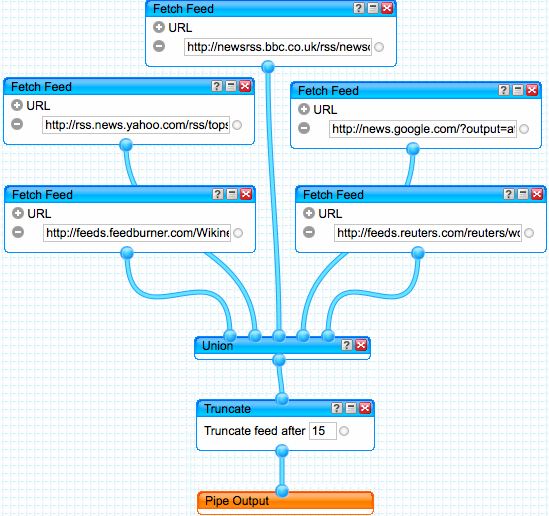
\includegraphics[width=\columnwidth]{img/yp-1}
\label{fig:ypexample}
\end{figure}


\section{Smells in end-user programs}
\label{sec:smells}
Research into end-user language smells has had two approaches, which are not mutually exclusive.
The first approach is to take existing smells for OO programming languages, usually those defined by Fowler~\cite{Fowl1999}, and transform them to be applicable to the end-user environment \cite{Hermans2012inter,Hermans2012intra,Stolee2011,StoleeTSE2013, chambers2013smell}.
The second approach is to define smells tailored to the end-user environment.
This can be done by interviewing experienced end-users to see which smells they perceive \cite{chambers2013smell}, by looking at user reports like forum or newsgroup posts~\cite{badame2012refactoring,chambers2013smell}, or by analyzing publicly available repositories \cite{Stolee2011,StoleeTSE2013,Hermans2012intra}.

This section provides an overview of different smells that researchers have found to be applicable to end-user artifacts using both the above described approaches and proposes future directions for smell detection in these domains. 

\begin{table*}
\caption{Code Smells in End-User Programs
\label{table:oosmellslarge}}
\centering
\sffamily
\begin{tabular} {@{}llll@{}}
\toprule
\textbf{OO Smell}
	& \textbf{Excel}
	& \textbf{Yahoo!\ Pipes}
\\ \midrule
Dead Code
	& %~\ding{55}
	& Unnecessary Module \cite{StoleeTSE2013}
\\ \cmidrule
Duplicate Code
	& Duplicated Formulas \cite{Hermans2012intra}
	& Duplicate Modules, Duplicate String or
\\ % Continuation
& 
& Isomorphic Paths \cite{StoleeTSE2013}
\\ \cmidrule
Feature Envy
	& Feature Envy \cite{Hermans2012inter}
	& %Feature Envy *
\\ \cmidrule
Inappropriate Intimacy
	& Inappropriate Intimacy \cite{Hermans2012inter}
	& %Inappropriate Intimacy *
\\ \cmidrule
Lazy class or Middle Man
	& Middle Man \cite{Hermans2012inter}
	& Unnecessary Abstraction \cite{StoleeTSE2013}
\\ \cmidrule
Long Method
	& Multiple Operations \cite{Hermans2012intra}
	& Noisy Module : Duplicate Field \cite{StoleeTSE2013}
\\ \cmidrule
Many Parameters
	& Multiple References \cite{Hermans2012intra}
	& 
\\ \cmidrule
Message Chain
	& Long Calculation Chain \cite{Hermans2012intra}
	& 
\\ \cmidrule
No-op
	& %Redundant Operations *
	& Unnecessary Module \cite{StoleeTSE2013}
\\ \cmidrule
Unused Field
	& %~\ding{55}
	& Noisy Module : Empty Field \cite{StoleeTSE2013}
\\ \cmidrule
Use of Deprecated Interfaces
	& %Deprecated Functions *
	& Deprecated Module or Invalid Source \cite{StoleeTSE2013}
\\ \bottomrule
%\multicolumn{4}{c}{} \\
%\multicolumn{4}{l}{\ding{55} : Not applicable due to the nature of the paradigm} \\
%\multicolumn{4}{l}{* : Proposed smell, likely future opportunity not supported by prior work}\\
%\multicolumn{4}{l}{$\langle$blank$\rangle$ : Not discussed in this work, possible future opportunity} \\
%\multicolumn{4}{l}{\todo{fill all empty spots, they should either be explicitly NA or possible}} \\
\end{tabular}
\end{table*}



%\subsection{OO Smells in End-User Programs}
%\label{sec:smells:oo}
 We summarize the OO smells present in two end-user languages, Excel spreadsheets and Yahoo!\ Pipes mashups, in Table~\ref{table:oosmellslarge}.
 Overall, we often observe similarities in the code smells studied. For example, the \emph{Duplicate Code}, \emph{Lazy Class}, and \emph{Long Method} smells  have been studied in both languages. 
% \todo{is this a fair assesment?}
We note that the absence of an entry in Table~\ref{table:oosmellslarge} does not mean the absence of the smell in that language, it simply means such smells have not been studied. We speculate on a few of these opportunities in Section~\ref{subsec:futuresmells}. 

% Some smells, like the \emph{Long Method} smell, have been studied in only one domain but are likely applicable in the other domain, these are marked with *.  These smells present opportunities for future research, detailed in Section~\ref{subsec:futuresmells}.
 
% In this section we will detail the application of OO smells on specific end-user languages.
 
% A small number of smells are definitely not applicable (\ding{55}) because of differences in the domains. Spreadsheets, for example, cannot contain dead code because the user might still be interested in a piece of data even if it is not used anywhere else in the spreadsheet.

 \subsection{Excel}
Hermans et al. \cite{Hermans2012inter,Hermans2012intra} analogize a workbook to a program, a worksheet to a class inside that program and a cell to a method and use this to transform nine of Fowlers smells.
An example of this is the \emph{Long Method} smell, which translates to the \emph{Multiple Operations} smell because formulas with a large number of operations suffer from similar problems as long methods. In an industrial case study with 10 spreadsheet users, the smells were found understandable by users, and with the smells errors in real-life spreadsheets were found.

\subsection{Yahoo!\ Pipes}
Stolee and Elbaum~\cite{Stolee2011, StoleeTSE2013} treat a Yahoo!\ Pipes mashup as a class and each module as a method.  Fields in a module are treated as parameters. Using this analogy,  several OO smells were mapped to this language. The most common smell, appearing in nearly one-third of the 8,000 pipes studied, was \emph{Duplicate Strings}, an instance of Fowler's \emph{Duplicate Code} smell. 
\emph{Duplicate Modules}, impacted nearly one-quarter of the pipes studied. 
 Overall, 81\% of the programs studied from the Yahoo!\ Pipes community had at least one smell. 
 
Yahoo!\ can also \emph{deprecate modules}, which can create similar problems to using deprecated or old versions of interfaces.


\begin{figure} [ht]
\caption{The interface of \ms~showing a simple line following program.}
\centering
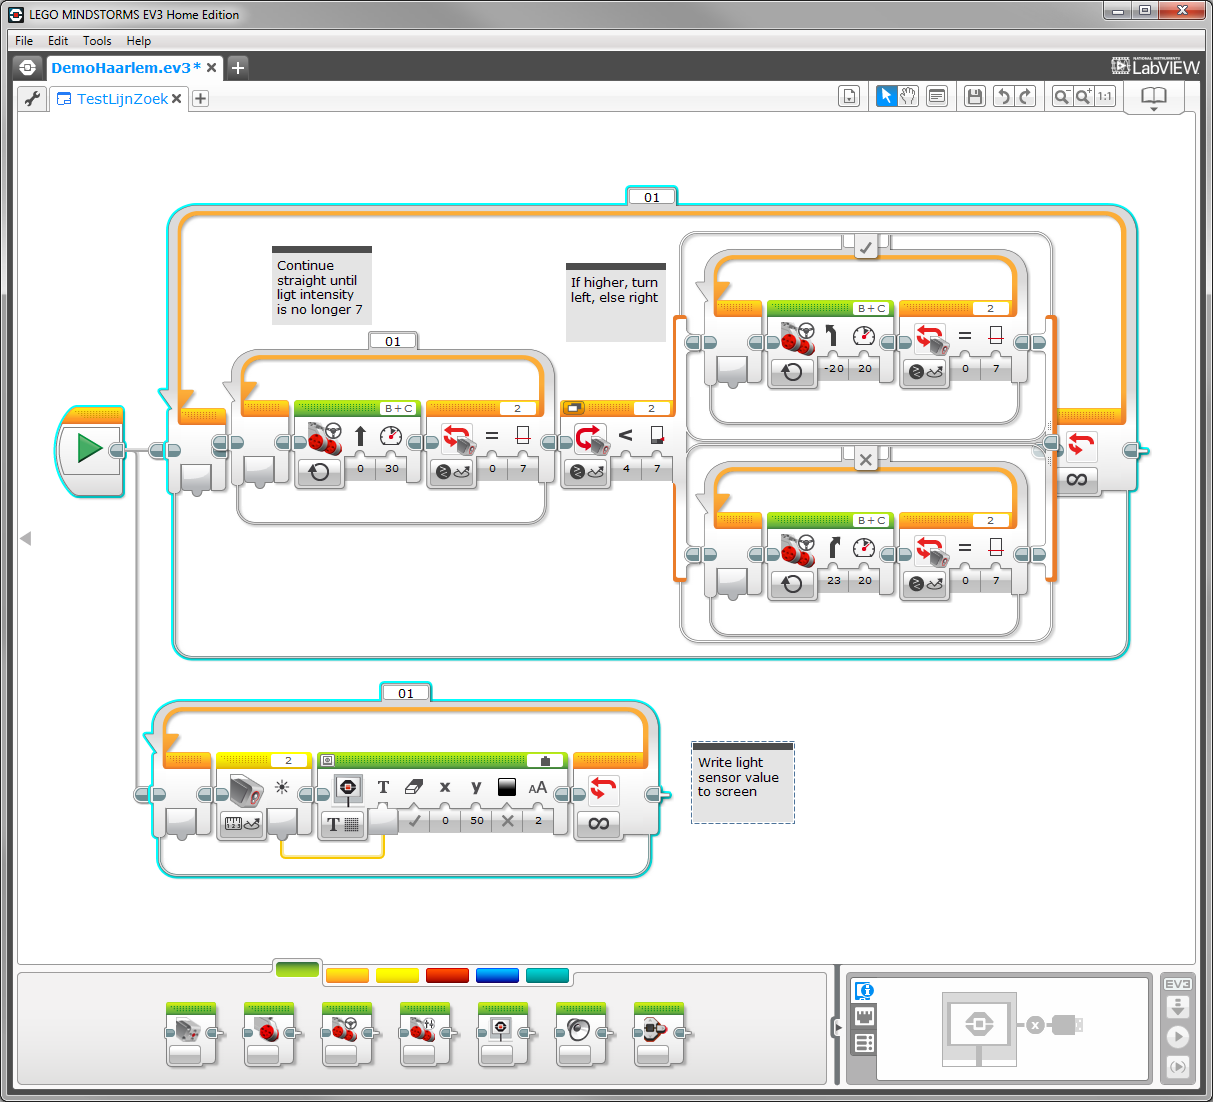
\includegraphics[width=\columnwidth]{img/ms}
\label{fig:ms}
\end{figure}


\section{Application}
\label{sec:application}
In Section~\ref{sec:smells}, we distill a catalog of end-user smells from previous work. In order to demonstrate the applicability of our catalog, we apply it to two new domains: \ms~software (EV3 for short) and  Kodu. 

\subsection{\ms}
\ms~is the third iteration of the LEGO MINDSTORMS robotics line. It consists of a number of sensors, four motors and an ARM 9 ``intelligent brick''. The robotics kit comes with a control software package, which allows for visual programming of the brick. The software supports several basic constructs common to programming, including loops and conditionals, but also more advanced features like parallel execution. Figure \ref{fig:ms} shows the user interface of the EV3 software with a program that makes a robot follow a black line by steering left if the sensor value is below the threshold of 7 and right if the value is above, and in parallel writes the sensor value to the screen. Blocks have to be connected by wires, like the two coming from the `Play button' that acts as the starting point, to be executed. The program in Figure \ref{fig:ms} demonstrates some of the basic EV3 programming concepts including parallel execution, loops and switches.

In addition to the programming concepts described above, users have the possibility to define `\mbs' which basically are subroutines. \mbs~may have up to 9 different input and one output parameter. \mbs~cannot be programmed from scratch; they can only be created by selecting blocks in an existing program and creating a new block for them, together with a call to the newly created block, an action extremely similar to `extract method' present in most modern IDEs. 

\subsubsection{Smells  in \ms}
In this subsection we describe how the smells in our OO-inspired catalog apply to EV3 programs. As common in the other approaches, we define a loose mapping of OO concepts to the end-user language in question to be able to translate the smells. In EV3 programming, there are  \emph{\mbs~} that contain a number of blocks, can be used multiple times and can use input and output. As such they resemble methods in source code, modules in Yahoo! Pipes and worksheets in spreadsheets. Based on this translation, we investigate which of the smells in our catalog could apply to EV3 programs too. 

\begin{description}
\item[Dead Code] It is possible for programming blocks to be disconnected, but the interface clearly indicates this by making them gray \todo{added picture here?}. However, unused \mbs~can be present in the project without a warning being issued. This is smelly as it makes the program unnecessarily large.
\item[Duplicate Code] When the same, or very similar combinations of blocks occur, this would be the duplicate code smell.
\item[Feature envy] While all defined variables within EV3 programs are global, they can be written in a certain \mb~but read in a different one. If, in a given \mb~many variables are read that have been written somewhere else, this might be an occurrence of the feature envy smell. 
\item[Inappropriate Intimacy] Variables might be read in one \mb~but written somewhere else. If there are two \mbs~sharing multiple variables this way, it might be better to combine them.
\item[Lazy Class] If a \mb~is very small, for example, consisting of just one block, they do not add a lot of value, while making the program harder to understand, as a user has to navigate to the \mb~to see what its function is.
\item[Long method] If a \mb~grows very large, it will no longer be easy to understand, counteracting the added value of the abstraction.
\item[Many Parameters] \mbs~can have 9 different parameters, which could be considered too much for easy understandability, especially since parameters need to be connected with wires, potentially leading to visual clutter in the case of many parameters.
\item[Message Chain] Because \mbs~can have both input and output parameters, it is possible that they created a message chain in which values are continuously passed until they are used, while they could have been passed outside of the \mbs~.
\item[No-op] It is possible to combine blocks in such a fashion that they do not actually contribute to the functionality of the program. For example, it a user stops the same motor twice, the second stop will be a no-op.
\item[Unused Field] As explained above, \mbs~can define parameters. However, the user is not forced to use them, hence it is possible to define more parameters than used.
\item[Use of Deprecated Interfaces] This is a smell that does not apply, as, to date, there is only one version of the EV3 software and no blocks have been depreciated.
\end{description}


\begin{figure} [ht]
\caption{Two blocks representing the same functionality, one in a regular block and one using a \mb.}
\centering
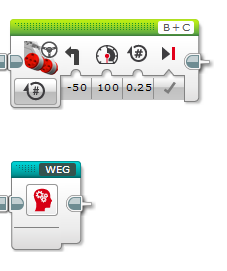
\includegraphics[width=3cm]{img/weg}
\label{fig:weg}
\end{figure}

\subsubsection{Study context}
To determine if EV3 programs indeed suffer form the above defined smells, we have gathered 17 programs from two data sources. The first source is robotics club ran by one of the authors of this paper. It is a club where kids aged 8 to 13 program robots every week. Their programs have been collected as dataset for this paper. More specifically, we focus on two different projects within this set, RoboCup and Sumo. These two types of programs related to two different LEGO MINDSTORMS competitions: Sumo is a simple robot game in which robots have to `sumo wrestle' each other: the robot that gets pushed out of the circular competition area first loses\footnote{\url{http://www.sugobot.com/}}. The Robocup programs were made to participate in the RoboCup Junior Rescue challenge\footnote{\url{http://rcj.robocup.org/rescue.html}}, where robots have to first navigate part of the field by following a line and subsequently look for a soda can and push it out of the field.

To obtain a more diverse set of EV3 programs, we have solicited members of the EV3 programming group on Facebook to share their programs with us\footnote{\url{https://www.facebook.com/groups/legomindstorms/permalink/527560164058881/}}.

\subsubsection{Findings}
When investigating the programs, we found that they indeed can suffer from OO-inspired smells. There are only two smells that do not occur in any of the programs: Inappropriate Intimacy and Message Chain. Duplicate Code occurs most, in over half of the programs. 

Table \ref{tab:robotica} presents an overview of the smells found in the EV3 programs.


\begin{figure} [ht]
\caption{The project properties screen for the Sumo program 1, showing the three \mbs~, but not indicating the \mb~`draaien' is currently not called from the main program.}
\centering
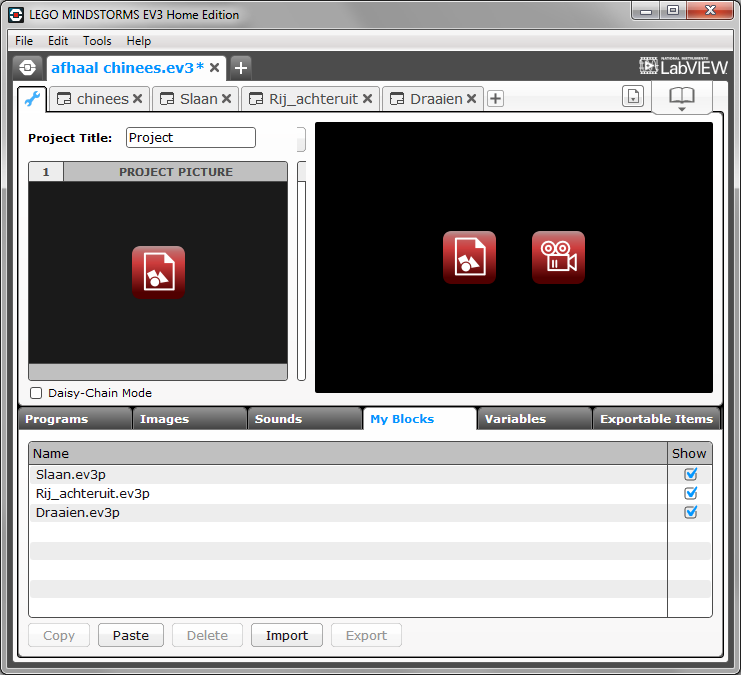
\includegraphics[width=\columnwidth]{img/overview}
\label{fig:overview}
\end{figure}

\paragraph{Duplicate Code}
The most common smell we found in the nine programs is the Duplicate Code smell, which 11 out of 17 programs suffer from. \todo{Add an example here?}

\paragraph{Dead Code}
The second most common smell is Dead Code. In seven out of 17 programs we found \mbs~that no longer connected to one of programs. This can pose a problem, as the EV3 environment compiles and transfers all programs and \mbs~to the brick, causing the memory to be full quite quickly. We see that Dead Code is more common in the robotics class programs than in the programs we received via Facebook. This is probably due to the fact that these users felt confident enough to share their programs, because either the programs were reviewed before sharing them, or the experience users selected `nice' programs to share.

Looking at the EV3 programming interface, it is not that surprising that users forget about disconnected \mbs. The interface does not help users in understanding what \mbs~are used. If we look at the project properties screen, shown in Figure \ref{fig:overview}, one can see that there is no information about which \mb~is used where. Even worse, user can delete \mbs~that are still being called, without a warning being issued about this. After removal of a \mb~ in use, the program no longer compiles.

\begin{table*}[]
\centering

\caption{Size in terms of the different number of blocks used in the seventeen \ms~programs, and the smells they exhibit}
\label{tab:robotica}
\sffamily
\begin{tabular}{l|lllll|lll|lllllllll}
Name & L1  & L2 & L3  & L4  & L5  & L6  & L7  & L8  & L9  & L10 & L11 & L12 & L13 & L14 & L15 & L16 & L17 \\
\hline
Data         & 1  & 0  & 2  & 5  & 0  & 0  & 4  & 4  & 1  & 0  & 0 & 2  & 0  & 7  & 1 & 1  & 0   \\
Actor        & 8  & 6  & 5  & 7  & 16 & 8  & 10 & 16 & 10 & 1  & 2 & 1  & 7  & 15 & 2 & 2  & 78  \\
Sensor       & 1  & 0  & 0  & 2  & 1  & 0  & 8  & 10 & 4  & 1  & 0 & 1  & 0  & 4  & 2 & 0  & 0   \\
Logic        & 3  & 5  & 4  & 4  & 4  & 3  & 7  & 11 & 2  & 2  & 1 & 4  & 11 & 2  & 0 & 0  & 25  \\
MyBlock Call & 2  & 0  & 2  & 2  & 3  & 4  & 3  & 5  & 0  & 1  & 0 & 1  & 0  & 3  & 1 & 4  & 27  \\
Comment      & 2  & 0  & 0  & 1  & 0  & 0  & 1  & 0  & 0  & 6  & 6 & 0  & 15 & 0  & 0 & 7  & 13  \\
Variables    & 0  & 0  & 1  & 3  & 1  & 1  & 0  & 0  & 0  & 0  & 0 & 0  & 0  & 19 & 0 & 0  & 0   \\
MyBlocks     & 3  & 0  & 3  & 2  & 3  & 2  & 2  & 4  & 0  & 1  & 0 & 1  & 0  & 4  & 1 & 3  & 6   \\
\hline
Total        & 20 & 11 & 17 & 26 & 28 & 18 & 35 & 50 & 17 & 12 & 9 & 10 & 33 & 54 & 7 & 17 & 149\\
\hline
\hline
Feature Envy                                           & \ding{51} &  & \ding{51} & \ding{51} &   &   &   &   &   &   &   &   &   &   &   &   &   \\
Long method                                            &   &  &   &   & \ding{51} &   &   &   &   & \ding{51} &   &   &   & \ding{51} &   &   & \ding{51}   \\
Inappropriate Intimacy                                 &   &  &   &   &   &   &   &   &   &   &   &   &   &   &   &   &   \\
Lazy Class                                             & \ding{51} &  & \ding{51} & \ding{51} &   & \ding{51} &   &   &   &   &   &   &   &   &   &   &   \\
Message Chain                                          &   &  &   &   &   &   &   &   &   &   &   &   &   &   &   &   &   \\
Many Parameters                                        &   &  &   &   &   &   &   &   &   &   &   & \ding{51} &   &   &   &   &   \\
Duplicate Code                                         &   &  &   & \ding{51} & \ding{51} & \ding{51} & \ding{51} & \ding{51} & \ding{51} & \ding{51} & \ding{51} &   & \ding{51} &   &   & \ding{51} & \ding{51} \\
Dead Code                                              & \ding{51} &  & \ding{51} & \ding{51} &   &   & \ding{51} & \ding{51} &   &   &   &   &   & \ding{51} &   &   & \ding{51} \\
Unused Field                                           &   &  &   & \ding{51} &   &   &   &   &   &   &   &   &   & \ding{51} &   &   &   \\
No-op                                                  &   &  & \ding{51} &   &   &   &   &   &   &   &   &   &   & \ding{51} &   &   &  \\

\end{tabular}
\end{table*}


\paragraph{Lazy Class}
Lazy classes, which we counted as \mbs~containing three or fewer blocks, are also relatively common, occurring in four of the programs. However, we only find this smell in the programs from the robotics club and not in the programs received via Facebook. Many of `lazy \mbs'~were relatively small, consisting of two or three blocks, or even one in some cases. You could say this is smelly, as understanding the \mb~requires clicking it and that might not be worth it for small \mbs. However, the EV3 programming interface does not allow regular blocks to be named, but it does allow this for \mbs. So by making a \mb, users can express the intent of a coherent set of blocks, even if this set consist of just one block. 

As an example, consider the two blocks shown in Figure 5, where the upper one is regular block controlling a motor, while the lower one is a call to a \mb~with the same functionality. The first one just expresses what the robot must do, but the second one expresses the intent (`weg' meaning flee). By using the \mb, even with one block, the program gets easier to read.

\paragraph{Long method}
Long Method too occurs in four programs, but, contrary to Lazy Class, is found mostly in the Facebook programs. This is to be expected, more experienced users can handle bigger \mbs, while the kids from the robotics club stick with making small blocks.

\subsubsection{Summary}
To summarize, we again observe that smells stemming from OO are applicable to end-user domain: duplicate code, dead code and small abstractions seem to be anti-patterns that occur in programming in general, independent of the programming language. It is interesting to see that even in a visual language, quite different from the textual, high-level languages for which the smells were originally designed, the same smells occur \todo{this seems to be a very worthwhile contribution/observation, should be repeated in abstract and conclusion}


\subsection{Kodu}
Microsoft Research's Kodu is a visual programming language~\cite{kodugrammar} and environment that allows users to create, play, and share their own video games. 
It is available for download on the Xbox and PC and is heavily inspired by robotics, and the context of programming in it and its language both show this. 
Users can program each character or object (e.g., a kodu, cycle, apple, tree; we use character and object interchangeably) individually, and the programming defines how to interact with the world. Each object has 12 pages that can be programmed, analogous to methods in an OO language, where the current page defines the current behavior of the object. 
The object's behavior can change by switching between pages to modify state and control flow. 
Each page contains a set of rules, and each rule is in the form of a condition and an action, which form a when~--~do clause. The \emph{when} is defined by a sensor (e.g., see, hear, gamepad input) and filters (e.g., apple, gamepad A button). The \emph{do} is defined by an actuator (e.g., movement, shoot) and modifiers (e.g., missile, toward). All the rules on a page are evaluated in a single frame, from top to bottom. 
Despite its unique language, Kodu  can be used to express many basic concepts in computer science, such as variables, boolean logic and conditional control flow~\cite{Stolee:2011:ECS:1953163.1953197}. 

Figure~\ref{fig:Kodu} shows a page and two rules  in Kodu. For the first rule, the condition is, when see red apple, and the action is, move toward it. The action defines the behavior of this particular character when it sees a red apple, that is, it moves toward it. Since the condition identifies an object (i.e., apple), it becomes the default selector, even though it is not explicitly specified. The second rule has a similar condition with a different sensor, bump. The action of the second rule, eat, indicates that the character should eat any red apple it bumps. The programming in Figure~\ref{fig:Kodu} applies to the first page in this character's programming, as indicated by the number one at the top of the screen. The first page is the default start page.


\begin{figure}[ht]
\caption{The interface of Kodu~showing programming behavior for a bot.}
\centering
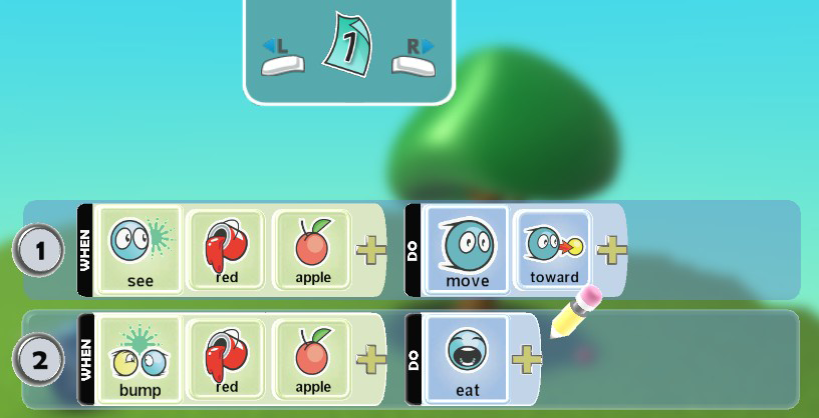
\includegraphics[width=\columnwidth]{programmingui.png}
\label{fig:Kodu}
\end{figure}



\subsubsection{Smells in Kodu}
We describe how the smells in our OO-inspired catalog apply to Kodu programs. We define a loose mapping of the OO concepts to the end-user language. We consider pages of programming as analogous to methods or classes, similar to how modules are treated in Yahoo!\ Pipes, worksheets in spreadsheets and \mbs~in \ms. 

\begin{description}
\item[Dead Code] If there exists a page with programming such that there is no explicit path of control flow from Page~1 to it, it is unreachable and therefore dead. 
\item[Duplicate Code] Two pages for the same character with exactly the same set of rules, or two identical rules on a page constitute duplicate code. Alternatively, two rules on the same page with the same sensor and filter but different actuators could be consolidated using a tabbed feature \todo{you did not introduce `tabbed' before} and are smelly. 
\item[Feature envy] All global variables, such as game scores, can be read and written by any character. If a certain character reads variables that have been written by another character, this could be an instance of the feature envy smell. 
\item[Inappropriate Intimacy] A character has four local properties that describe its state: color, glow color, expressions (angry, crazy, happy). If one character frequently checks the properties of another character, this could constitute inappropriate intimacy. 
\item[Lazy Class] If a character has no programming, it could be an instance of the lazy smell. 
%Characters with no programming are different than objects. Characters can have movement whereas objects cannot. 
\item[Long method] A page with many, many rules may be difficult to understand. Some programming could potentially move to other pages or other characters. We counted long methods as those with more than five rules. 
\item[Many Parameters] A game can have 37 different global scores. Games that use many of these could be unnecessarily smelly. 
\item[Message Chain] It is possible for a character to create a chain of switches between pages without any logic on the page other than the jump. This would create a long and unnecessary message chain. 
\item[No-op] Jumping to a page with no logic is the logical equivalent of a null pointer. While no error would be raised, the character would no longer have any behavior and would be stuck in that state. Alternatively, rules with 'when' clauses but no 'do' clauses do not perform any actions. 
\item[Unused Field] A global variable that is written to but not read is an instance of the the unused field smell. 
\item[Use of Deprecated Interfaces] Some language features and bots may exist in early versions of Kodu but not be available in future versions. use of these deprecated entities may cause unexpected behavior when running an old program in a new environment and be smelly. 

%\todo{emailed scoy at Microsoft about this}
\end{description}



\begin{table*}[]
\centering

\caption{Size in terms of the different number of characters and rules used in the 17 Kodu programs, and the smells they exhibit}
\label{tab:koduanalysis}
\sffamily
\begin{tabular}{l | lllllllllllllllll}
Name & K1  & K2 & K3  & K4  & K5  & K6  & K7  & K8  & K9  & K10 & K11 & K12 & K13 & K14 & K15 & K16 & K17 \\
\hline
Actors        & 6&17&39&21&62&60&85&26&26&60&42&45&57&36&5&15&28\\
Pages 		&11&7&26&19&18&47&82&19&10&60&41&31&10&9&6&7&7\\
Rules 		&21&17&60&28&31&96&93&29&20&120&58&63&22&35&14&18&23\\
%Tiles        	& 90&64&252&150&121&418&535&141&66&227&230&244&81&159&54&90&103\\
HCI Actors & 1&2&1&1&2&1&1&1&1&1&1&1&1&0&2&1&1\\
%\hline
%Total        & 20 & 11 & 17 & 26 & 28 & 18 & 35 & 50 & 17 & 12 & 9 & 10 & 33 & 54 & 7 & 17 & 149\\
\hline
\hline
Feature Envy                                         &   &  & \ding{51}  &   &   &   &   &   &   & \ding{51}  &   &   &   &   &   &   &   \\
Long method                                        &  &  &  &   &   &\ding{51}   & &   & &   &   & \ding{51}  & \ding{51}  &   &   &   &    \\
Inappropriate Intimacy                            &   &  &   &   &   &   &   &   &   &   &   &   &   &   &   &  \ding{51} &   \\
Lazy Class                                             &   & \ding{51} & \ding{51}  & \ding{51}  & \ding{51}  &\ding{51}   &\ding{51}   &\ding{51}   &\ding{51}   &   & \ding{51}  & \ding{51}  & \ding{51}  & \ding{51}  & \ding{51}  &  \ding{51} &\ding{51}   \\
Message Chain                                          &   &  &   &   &   &   &   &   &   &   &   &   &   &   &   &   &   \\
Many Parameters                                        &   &  &   &   &   &   &   &   &   &   &   &   &   &   &   &   &   \\
Duplicate Code                                        &   &  & \ding{51}  &   &   & \ding{51}  & \ding{51}  & \ding{51}  & \ding{51}  &   &   & \ding{51}  &\ding{51}   & \ding{51}  &   & \ding{51}  &   \\
Dead Code                                              &   &  &   &   &   &   &   &   &   &   &   &   &  \ding{51} &   &   &   &   \\
Unused Field                                           &   &  &  \ding{51} &   &   &   &   &   & \ding{51}  &   &   & \ding{51}  &   &   & \ding{51}  &   &   \\
No-op                                                  &   & \ding{51} &   &   &   &   &   &   &   & \ding{51}  &   & \ding{51}  & \ding{51}  & \ding{51}  &   &   &\ding{51}   \\
\hline
Total Smells & 0 & 2 & 4 & 1 & 1 & 3 & 2 & 2 & 3 & 2 & 1 & 5 & 5 & 3 & 2 & 3 & 2 \\

\end{tabular}
\end{table*}


\subsubsection{Study Context}
To determine if Kodu programs indeed suffer form the above defined smells, we have gathered  programs from two data sources. 
We ran a workshop that introduced children to Kodu Game Lab in a series of three 3-hour sessions.  To recruit participants, we advertised the Kodu workshop using a mailing list of parents interested in Kodu.  Twenty-seven children (9 girls) between the ages of 9 and 12 volunteered to participate, with parental consent.

\subsubsection{Findings}


Analysis parameters:
\begin{itemize}
\item Long Method needs to have 10 or more rules
\item Many parameters needs 4 or more score buckets
\end{itemize}

\begin{table}
\caption{Summary of Smells Across EV3 and Kodu Programs \label{tab:smell summary}}
\begin{center}
\begin{tabular}{l | r r}
&Kodu&EV3\\ \hline
Feature Envy&22\%&18\%\\
Long method&25\%&24\%\\
Inappropriate Intimacy&4\%&0\%\\
Lazy Class&79\%&24\%\\
Message Chain&4\%&0\%\\
Many Parameters&36\%&6\%\\
Duplicate Code&61\%&65\%\\
Dead Code&11\%&41\%\\
Unused Field&25\%&12\%\\
No-op&41\%&12\%\\
\end{tabular}
\end{center}
\end{table}

\subsubsection{Summary}

\section{Future Opportunities for Smell Detection}
\label{sec:beyond}

\subsection{New Applications of OO smells}
\label{subsec:futuresmells}
Although not all OO smells have been studied in both domains, this does not mean they do not apply. For example, Feature Envy is not discussed in previous work on Yahoo! Pipes, but could apply when \todo{Katie, how exactly?}. Similarly, redundant operations could occur in Excel, in fact, they do. A formula like SUM(A1+A2+A3), that we have seen in practice, exhibits the No-Op smell. While the occurrence of these smells falls outside of the scope of the current work, in this section we discuss the potential of generalizing some of the OO and domain-specific smell definitions to additional domains, thus addressing all *'s in Table \ref{table:oosmellslarge}.

\subsubsection{Excel}
Most of the smells studied in other end-user domains have been studied in Excel spreadsheets, but there is some future potential in the areas of redundancy and deprecation.

Currently all research in smells and spreadsheets has focused on Microsoft Excel.
However, other spreadsheet software exists and operates on the same principles.
Thus there is an opportunity to confirm that the identified smells apply in other spreadsheet software.

\subsubsection{Yahoo!\ Pipes}
\label{sec:smells:future:yp}
%Many of the smells studied in Excel and LabVIEW could apply to Yahoo!\ Pipes, and in particular, \emph{Feature Envy} and \emph{Inappropriate Intimacy}. 
%uses methods of another class excessively - envy
The \emph{Feature Envy} smell could  apply when introducing abstraction. For example, if a pipe has several instances of the same subpipe module, this could be excessive use of another class. 

%depends on implementation of another class too much - intimacy
When a program uses too much abstraction relative to the size of the pipe, it could suffer from \emph{Inappropriate Intimacy} by depending too much on the implementation of the other class. In fact, in an empirical evaluation, programmers often preferred pipes without subpipe modules because they were easier to understand~\cite{StoleeTSE2013}. 

%long method
A \emph{Long Module} smell could apply when a module has a large number of fields. For example, the \emph{Fetch Feed} module, as in Figure~\ref{fig:ypexample}, can hold one or more URLs. When the number of URLs makes the method so big it does not fit on the screen, this would likely impact the understandability of the pipe. 

Drawing inspiration from the domain-specific \emph{Inconsistent Formula} smell in Excel, identifying program patterns that are close, but not exactly the same, could identify missed opportunities for abstraction or errors in the mashup structure. 


%\subsubsection{Other Domains}
%End-user programming domains extend beyond spreadsheets and web mashupss. Stolee and Elbaum explore future opportunities for refactoring in educational programming languages~\cite{StoleeTSE2013}. \todo{revisit, this is a bit strange now this paper talks about education too}

%Other end-user programming domains that could benefit from smell analysis and refactoring are mathematical environments like MATLAB, Sage, and Mathematica.

%In particular, the smells related to duplication and poor construction like \emph{Long Method}, \emph{Many Parameters} and \emph{Dead Code} are prevalent in the four domains studied.
%These smells -- and their respective refactorings -- likely exist in other end-user programming domains, and likely hinder the understandability and maintainability of those programs. Worse even, these smells could lead to errors, and thus these smells are worthy of our attention. 

%\subsection{Future Opportunities in Professional Languages}
%In end-user programming languages, it has been shown that code smells impact the understandability of
%source code~\cite{StoleeTSE2013}. Additionally, being presented with code smells can motivate end-user programmers to improve their code~\cite{chambers2013smell}, and smells in spreadsheets have even been known to reveal actual errors~\cite{Hermans2012intra}. These lessons could extend to professional programming languages. but further study is needed. 
% outside of the end-user programming domains. 
%There has been successful in using automating smell detection, for example, during agile development (e.g.,~\cite{Schumacher:2010:BES:1852786.1852797}). Paired with the end-user evidence, a stronger case can be made to integrate automated smell detection in many domains. 

%\todo{Other data flow languages could benefit from \emph{normalize order of operations} to improve understandability (as it does with YP). }

\subsection{Beyond OO}
\label{sec:smells:domain}
The end-user programming environments offer many opportunities to define smells based on user behavior or unique elements of the domain. Here, we explore opportunities for new smells in end-user domains that extend beyond the OO-inspired smells in Section~\ref{sec:smells}. 

\subsubsection{Excel}

In spreadsheets data is often processed by having each record in a row and having a column with identical formulas to perform some calculation.
This leads to the definition of the \emph{Inconsistent Formula} smell, which occurs if a single, or small number, of cells contain a different formula while its neighbors or other cells in the row or column contain an identical formula.
Interestingly this smell is already detected by Microsoft Excel which warns the user about it.

Another smell specific to spreadsheets is when a formula references an empty cell, which is often in error \cite{cunha2012towards}.
This is comparable to a null pointer in other languages and would be a runtime error, but because a spreadsheet contains both the input data and logic we can directly mark it as a smell.

\subsubsection{Yahoo!\ Pipes}
%Talk about smells unique to the domain
By exploring a large subset of the Yahoo!\ Pipes repository, Stolee and Elbaum identified a smell based on the presence of broken data sources~\cite{StoleeTSE2013}.
A reference to a broken data sources  is similar to opening a non-existing file, which would be a runtime exception or error in most professional languages.
Such exceptions are not in the Yahoo!\ Pipes language, which is the reason to mark it as a smell. 
%Talk about deriving smells from the community
Similar exploration was used to  identify common programming practices, marking deviations from those practices as smells. 
This is similar to identifying  smells  as anti-patterns  and could be extended to any language. 

\subsubsection{EV3}

\subsubsection{Kodu}

\section{Related Work}

\label{sec:related_work}
This paper builds upon the extensive body of work related to code smells and refactoring in the end-user programming domain~\cite{Stolee2015, Stolee2011, StoleeTSE2013, Hermans2011, Hermans2012intra, Hermans2012inter, hermans2014bumblebee, chambers2013smell, chambers2015impact}. For an extensive overview in object-oriented research, we refer the reader to the work of Mens and Tourw\'{e} \cite{mens2004survey}.

\subsection{Smells based on user input}
\label{subsec:related_datasmells}
In end-user programming environments user input and logic are often more closely linked than they are in general purpose languages.
As such analyzing the input data as opposed to the logic can also be used to detect problems.

Cunha et. al \cite{cunha2012towards} claim to define code smells for spreadsheet, but for most of their smells they look at  anomalies in the data and define these as smells.
Examples of this are \textit{Standard Deviation} which occurs if one assumes a normal distribution for a column in numeric values and the column contains values which fall outside two standard deviations.
In more recent work, Barowy et. Al \cite{barowy2014checkcell} take a  more formalized approach which they label ``Data Debugging''.
Their solution uses statistical analysis to find values with an unusually high impact on the calculated results in a spreadsheet, as such values are likely either very important or erroneous.





\section{Discussion}
\label{sec:discussion}

Based on the research and results for smell detection in end-user programming domains, there are many directions for future work in the domains studied and other end-user domains.





\subsection{Threats to Validity}
The threats to validity of this work inherit the threats to validity of the original studies~\cite{Stolee2015, Stolee2011, StoleeTSE2013, Hermans2011, Hermans2012intra, Hermans2012inter, hermans2014bumblebee, chambers2013smell, chambers2015impact, badame2012refactoring}.

The three domains studied in this paper all happen to be dataflow languages, and the smells and refactorings may not generalize to other end-user programming domains (e.g., Scratch is OO-based). 

In addition, we note that the authors of this work have pioneered smell detection and refactoring research in spreadsheets and Yahoo!\ Pipes, but are not involved with LabVIEW. Thus, the opportunities for future work in this area may not be complete.  

\section{Concluding Remarks}
\label{sec:conclusions}
This paper presents an overview of the work in smell detection for end-user programming languages. More specifically, it synthesizes work on Yahoo!\ Pipes and Excel into a catalog of generally applicable smells in end-user languages. To demonstrate the applicability of the catalog, we apply it to two new domains: \ms~and Kodu, two visual languages aimed at programming education. The results show that indeed many of the catalog's smells apply in the new domains, and small abstractions, duplicate code and dead code occur in these educational languages too, while being of a quite different character than the textual languages aimed at professional developers that the smells were originally defined for. This shows the applicability of these smells but also warrants further research into issues end-users encounter while programming. The contributions of this paper are:

\begin{itemize}
	\item A catalog of object-oriented-inspired code smells in end-user programs (Section \ref{sec:smells})
	\item Application of the catalog to two new end-user domains focused on education (Section \ref{sec:application})
	\item Identification of future opportunities for smell detection in end-user programming domains, both within and beyond the OO paradigm (Section \ref{sec:beyond})
\end{itemize}

The current work gives rise to more research, for example \todo{future work}


\balance

\section*{Acknowledgements}
Special thanks to Stephen Coy for his help with Kodu. This work is supported in part by  NSF SHF-EAGER-1446932 and the Harpole-Pentair endowment at Iowa State University.


\bibliographystyle{IEEEtran}
\bibliography{literaturelist}

\end{document}


